\subsection{Convenience}
  \textbf{Infraestructura}. Por ejemplo, el almacenamiento. Los datos publicados son los mas recientes, por lo que no hay manera de obtener 
un historico de los datos si no son almacenados periodicamente. Una vez extraidos los datos, el usuario debera 
contar con una infraestructura que le permita almacenar los datos.
 \textbf{Automatizacion}. Este proceso tiende a ser arduo, por lo que sera necesario automatizarlo, de otra 
forma el esfuerzo requerido por el usuario para extraer la informacion no le compensara. 

Seguramente, realizaremos tareas repetitivas, como por ejemplo la representacion de los datos que son actualizados periodicamente.
Automatizacion para que se vea siempre lo que queremos
Estos procesos pueden llegar
a ser muy tediosos si no se automatizan.
Despues de seleccionar los campos necesarios deacurdo a nuestro diseno, se han realizado diferentes tareas de limpieza y transformacion,
como la eliminacion de datos no relevantes, por ejemplo el identificador de la estacion de medida, ya que el conjunto de datos
contiene las coordenadas de la estacion y para nosotros es mucho mas interesante.
Transformacion de campos a un formato adecuado, por ejemplo la fecha y hora en el que la medida ha sido tomada se almacena en formato fecha
en vez de cadena como se proporciona en el conjunto de datos en crudo.
Este conjunto de datos ofrece una o varias medidas por cada contaminante, que puede representarse por tres campos distintos, una medida 
cuantitativa, una cualitativa de la estacion fija de medida y una cualitativa de una estacion movil. Anadiremos un campo con la medida
mas relevante y eliminaremos las demas para minimizar el tiempo de procesado.

Por seguridad, se ha implementado una segunda arquitectura totalmente independiente que recolecta los datos y almacena en crudo.

Ademas proporcionaremos
la infraestructura necesaria para que el usuario solo tenga que consultar los datos y automatizaremos los procesos que deban repetirse
periodicamente.


\subsubsection{How to solve it} 
\subsubsection{How we solve it. Aire Guru} 
Se actualiza cada hora, por lo que si queremos acceder a unos datos en concreto, deberemos repetir la operacion periodicamente.
Un valor importante de este conjunto de datos es saber la evolucion de la polucion por zonas, la extraccion de esta informacion no es posible
si no se realiza un almacenado de los datos.

Aire Guru automatiza el proceso de recoleccion de los datos mediante un trabajo CRON que ejecuta un script implementado en JavaScript periodicamente. Este lee 
los datos de la url, los procesa, limpia y almacena en una base de datos MongoDB.

\begin{figure}[ht]
    \centering
    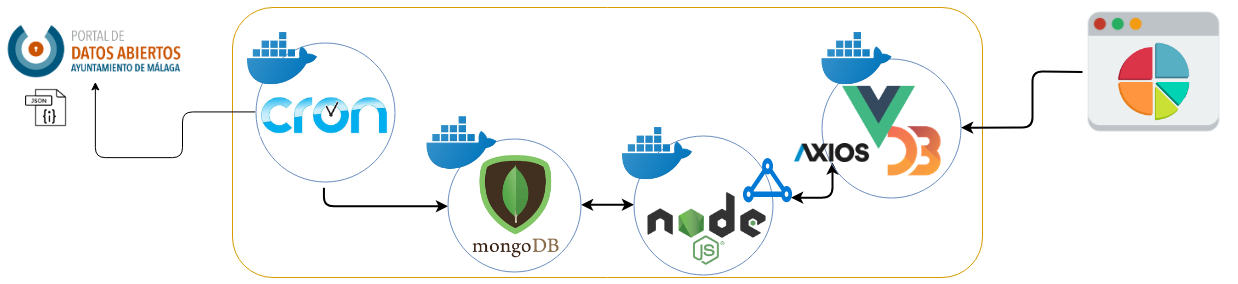
\includegraphics[width=12cm]{aireGuruArquitecture}
    \caption{Arquitecture Aire Guru}
\end{figure}

Mediante una interfaz web, muestra los datos al usuarios.

\begin{figure}[ht]
    \centering
    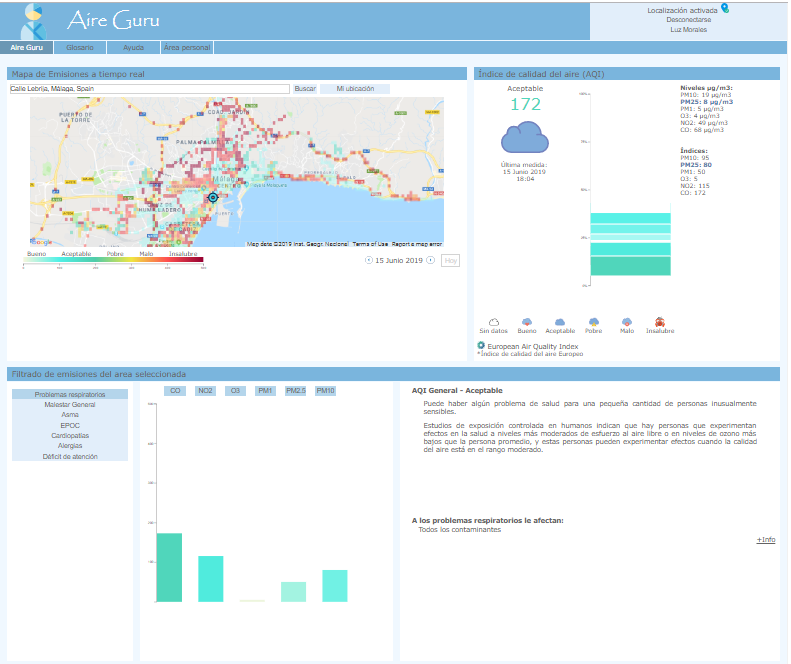
\includegraphics[width=9cm]{aireGuru}
    \caption{Aire Guru. Web Interface}
\end{figure}

\elsparagraph{Evaluation}  
\begin{itemize}
  \done Los datos necesarios para nuestro modelo han sido extraidos de los datos en crudo
\done Infraestructura. Implementa toda la arquitectura necesaria tanto de almacenaje, procesado como visualizacion.
\done Automatiza los procesos de recoleccion de datos y los calculos necesarios para mostrar la informacion al usuario. Por ejemplo, una pregunta simple 
seria saber a que nivel de polucion estamos rodeados en las coordenadas en la que nos encontramos. Con la informacion en crudo obtenida desde el portal, 
nos es una tarea imposible, pero si ardua si no contamos con un sistema que procese los datos. Aire Guru resulve este problema.
\end{itemize}